\section{离散无记忆信道}

信息论中最常用的是离散无记忆信道.

\subsection{离散无记忆信道的一般定义}

\textbf{1. 离散无记忆信源}

设 $ \mathscr{S}^{n}=\left\{\mathscr{X}^{n}, p^{(n)}\left(x^{n}\right)\right\} $ 是由 $ \mathscr{S}=(\mathscr{X}, p(x)) $ 确定的信源序列,如果对任何的 $ n=1,2,3, \cdots $,$x^{n} \in \mathscr{X}^{n}=\left\{x^{n}=\left(x_{1}, x_{2}, \cdots, x_{n}\right) \mid x_{i} \in \mathscr{X}\right\}$,有
$$
p\left(x^{n}\right)=p\left(x_{1}, x_{2}, \cdots, x_{n}\right)=\prod_{k=1}^{n} p\left(x_{k}\right)
$$
则称 $ \mathscr{S}^{n}=\left(\mathscr{X}^{n}, p^{n}\left(x^{(n)}\right)\right) $ 是由 $ \mathscr{S}=(\mathscr{X}, p(x)) $ 确定的无记忆信源序列.

\textbf{2. 离散无记忆信道}

记 $ \mathscr{C}^{n} $ 是一个信道序列, $ \mathscr{C}^{n}=\left(\mathscr{U}^{n}, p\left(v^{(n)}\right) \mid u^{(n)}, \mathscr{V}^{n}\right) $, 如果它的转移概率分布满足
$$
p\left(v^{(n)} \mid u^{(n)}\right)=\prod_{i=1}^{n} p\left(v_{i} \mid u_{i}\right)
$$
对 $ \forall u^{(n)}=\left(u_{1}, u_{2}, \cdots, u_{n}\right) \in \mathscr{U}^{n}, v^{(n)}=\left(v_{1}, v_{2}, \cdots, v_{n}\right) \in \mathscr{V}^{n} $都成立,其中 $ \mathscr{C}=(\mathscr{U}, p(v \mid u), \mathscr{V}) $ 是一固定的信道,则称 $ \mathscr{C}^{n} $ 是由 $ \mathscr{C} $ 决定的无记忆信道序列,或简称 $ \mathscr{C}^{n}(\mathscr{C}) $ 为无记忆信道.

\begin{remark}

    (1)离散信道指输入输出字母表均为离散事件集(有限的);

    (2) 无记忆指当输入字母 $ u_{i} $ 固定时, 它接收信号字母 $ v_{i} $ 的概率与以前、以后输入输出信号无关.
\end{remark}


\subsection{几种特殊的离散无记忆信道}

\textbf{1. 二元对称信道(无丢失)}

记输入输出字母表 $ \mathscr{U}=\mathscr{V}=\{0,1\} $. 信道转移概率分布为
$$
p(0 \mid 1)=p(1 \mid 0)=p, p(0 \mid 0)=p(1 \mid 1)=1-p
$$
称 $ p $ 为交叉概率误差 (输入 0 输出 1 和输入 1 输出为 0 )

\begin{figure}[h]
    \centering
    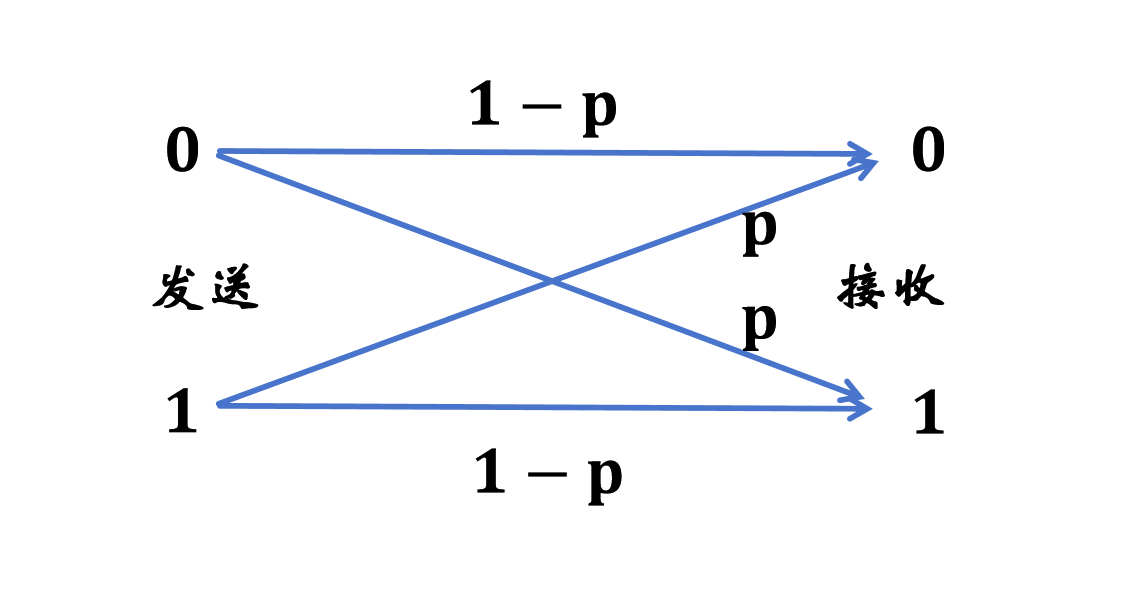
\includegraphics[width=.6\linewidth]{image/3.png}
    \caption{二元对称信道}
    %\label{fig:enter-label}
\end{figure}

信道转移概率矩阵为
$ \left(\begin{array}{cc} 1-p & p \\ p & 1-p\end{array}\right) $

\textbf{2. 二元擦除信道( $\mathrm{M}$ 信道)(有丢失)}

下图所示的信道称为二元擦除信道,输出*表示输入的丢失或擦除.

\begin{figure}[h]
    \centering
    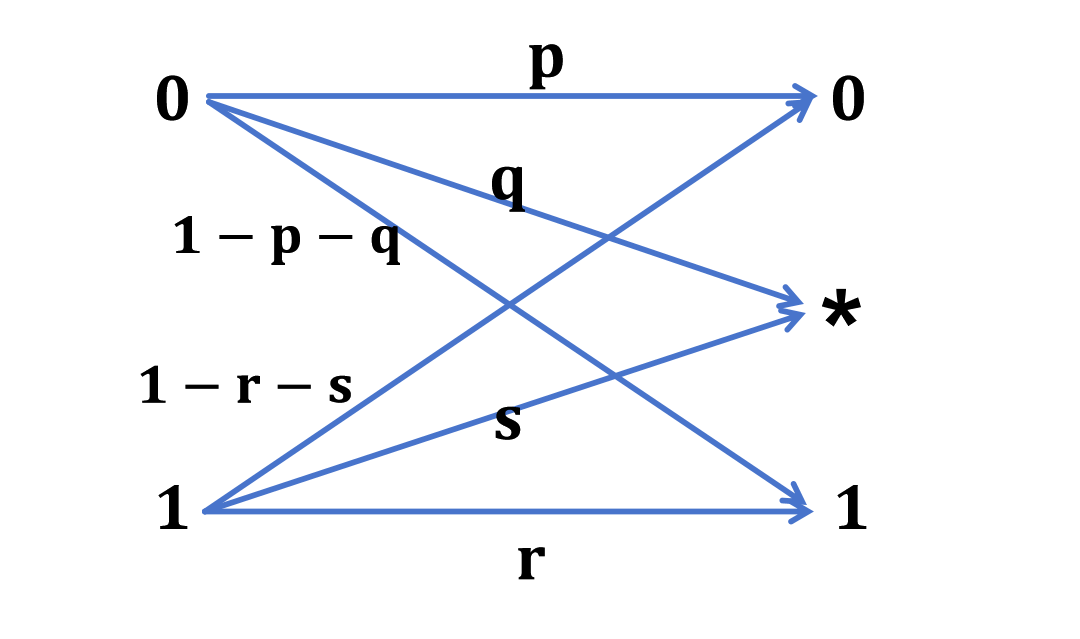
\includegraphics[width=0.5\linewidth]{image/4.png}
    \caption{二元擦除信道}
    %\label{fig:enter-label}
\end{figure}

二元擦除信道的一个特例如下图所示, 称之为 $ M $ 信道, 这个名字来源于它的图类似于字母 $ M $.
$$
p(0 \mid 0)=p(1 \mid 1)=1-p, p(* \mid 0)=p(* \mid 1)=p
$$
\begin{figure}[h]
    \centering
    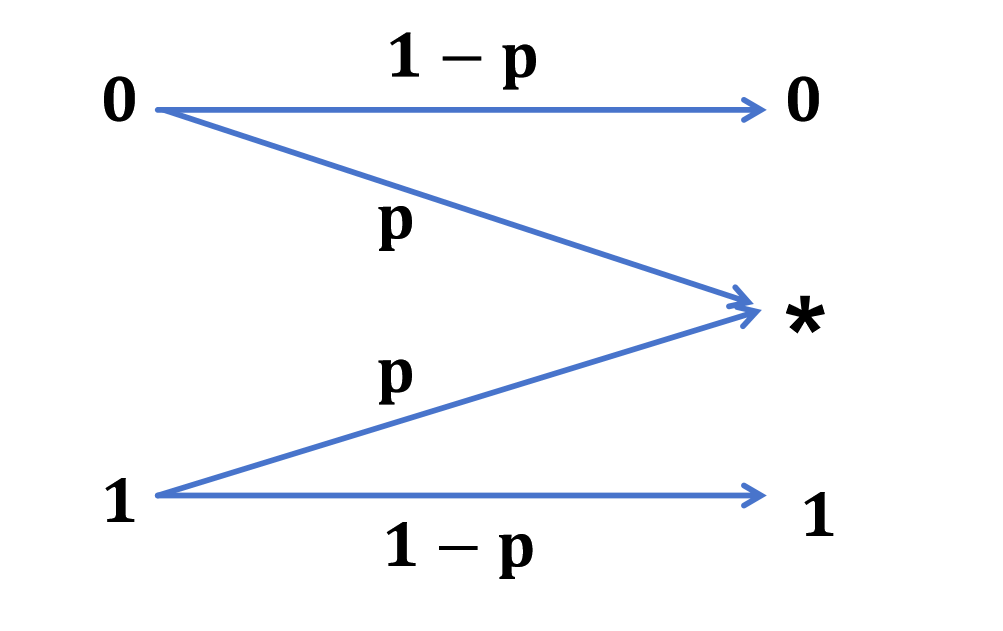
\includegraphics[width=0.5\linewidth]{image/5.png}
    \caption{$M$信道}
    %\label{fig:enter-label}
\end{figure}

\textbf{3. 信道转移概率矩阵} \textbf{(信道矩阵)}

设 $ \mathscr{U}=\left\{u_{1}, u_{2}, \cdots, u_{a}\right\}, \mathscr{V}=\left\{v_{1}, v_{2}, \cdots, v_{b}\right\} $, 定义信道矩阵为
$$
\left(\begin{array}{cccc}
p\left(v_{1} \mid u_{1}\right) & p\left(v_{2} \mid u_{1}\right) & \cdots & p\left(v_{b} \mid u_{1}\right) \\
p\left(v_{1} \mid u_{2}\right) & p\left(v_{2} \mid u_{2}\right) & \cdots & p\left(v_{b} \mid u_{2}\right) \\
\vdots & \vdots & & \vdots \\
p\left(v_{1} \mid u_{a}\right) & p\left(v_{2} \mid u_{a}\right) & \cdots & p\left(v_{b} \mid u_{a}\right)
\end{array}\right)
$$
是一个 $ a \times b $ 阶矩阵, 则该矩阵的每一行对应一个输入字母, 每一列对应一个输出字母,该矩阵的每一行元素之和为 1 , 即
$$
\sum_{j=1}^{b} p\left(v_{j} \mid u_{i}\right)=1, \quad i=1, \cdots, a
$$

按照信道矩阵, 可定义下面几种典型的离散无记忆信道.
\begin{figure}[h]
    \centering
    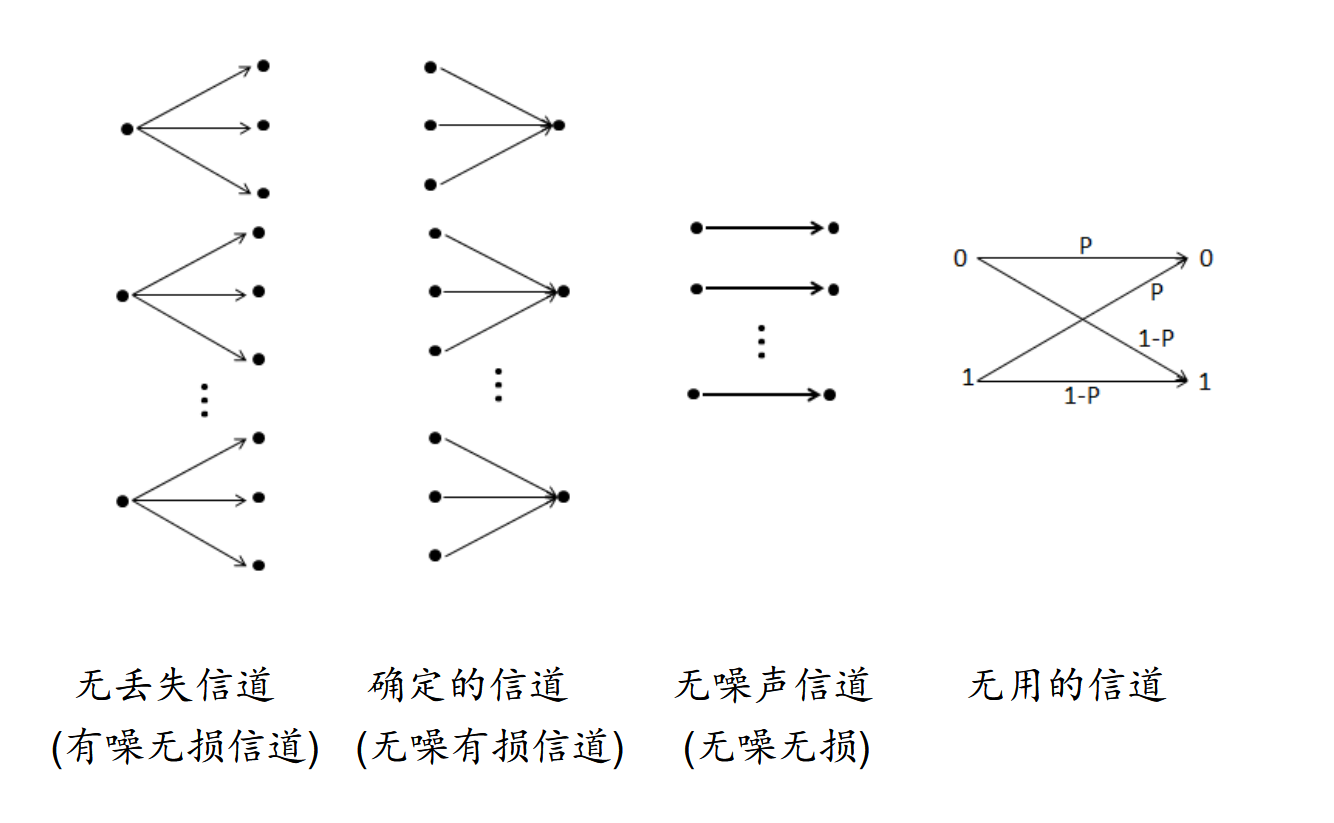
\includegraphics[width=.6\linewidth]{image/6.png}
\end{figure}

\begin{definition}
    (1) 如果输入 $ \xi $ 完全由输出 $ \eta $ 所决定, 称该信道是无丢失的.
    
(2) 如果输出 $ \eta $ 完全由输入 $ \xi $ 所决定,称该信道为决定的(确定的).

(3) 如果信道既是无丢失的也是决定的,称信道是无噪声的.

(4) 如果输入随机变量 $ \xi $ 的知识不能告诉我们任何关于输出 $ \eta $ 的知识,称其为无用的信道.
\end{definition}

\begin{definition}
    根据信道矩阵, 可以定义几种不同信道\\
(1) 如果信道矩阵的每一行是另一行的置换, 则称这个信道是行对称的.\\
(2) 如果信道矩阵的每一列是另一列的置换, 则称这个信道是列对称的.\\
(3) 如果信道矩阵是行对称的, 也是列对称的, 则称这个信道是对称的.
\end{definition}
 
\begin{example}
    具有信道矩阵 $ \left(\begin{array}{cccc}\frac{1}{3} & \frac{1}{3} & \frac{1}{6} & \frac{1}{6} \\ \frac{1}{6} & \frac{1}{6} & \frac{1}{3} & \frac{1}{3}\end{array}\right) $ 和 $ \left(\begin{array}{ccc}\frac{1}{2} & \frac{1}{3} & \frac{1}{6} \\ \frac{1}{6} & \frac{1}{2} & \frac{1}{3} \\ \frac{1}{3} & \frac{1}{6} & \frac{1}{2}\end{array}\right) $ 的信道都是对称的.

信道矩阵为 $ \left(\begin{array}{cccc}\frac{1}{3} & \frac{1}{3} & \frac{1}{6} & \frac{1}{6} \\ \frac{1}{6} & \frac{1}{3} & \frac{1}{6} & \frac{1}{3}\end{array}\right) $ 的信道是行对称的, 但不是列对称信道.
\end{example}

\textbf{4. 行对称信道和列对称信道的主要特征}

\begin{theorem}
     对于行对称信道, 知道 $ \xi $ 时 $ \eta $ 的不确定性与 $ \xi $ 分布无关, 即 $ H(\eta \mid \xi) $ 与入口分布无关.事实上,对任意 $ i=1,2, \cdots, a $, 我们有
$$
H(\eta \mid \xi)=\sum_{j=1}^{b} p\left(v_{j} \mid u_{i}\right) \log \frac{1}{p\left(v_{j} \mid u_{i}\right)}
$$
换句话说,一个信道是行对称的,如果给定输入 $ \xi $ 时关于输出 $ \eta $ 的知识并不依赖于所使用的入口分布.
\end{theorem}
\begin{proof}
    
\end{proof}
 $$ \begin{aligned}H(\eta \mid \xi)&=\sum_{i=1}^{a} p\left(u_{i}\right) H\left(\eta \mid \xi=u_{i}\right) 
=\sum_{i=1}^{a} p\left(u_{i}\right)\left(\sum_{j=1}^{b} p\left(v_{j} \mid u_{i}\right) \log \frac{1}{p\left(v_{j} \mid u_{i}\right)}\right)\\
&=p\left(u_{1}\right) \cdot \sum_{j=1}^{b}\left(p\left(v_{j} \mid u_{1}\right) \log \frac{1}{p\left(v_{j} \mid u_{1}\right)}\right)+p\left(u_{2}\right) \cdot \sum_{j=1}^{b}\left(p\left(v_{j} \mid u_{2}\right) \log \frac{1}{p\left(v_{j} \mid u_{2}\right)}\right) \\
&+\cdots+p\left(u_{a}\right) \cdot \sum_{j=1}^{b}\left(p\left(v_{j} \mid u_{a}\right) \log \frac{1}{p\left(v_{j} \mid u_{a}\right)}\right)
\end{aligned}
$$

因行对称,每行元素互为置换,故
$$
\sum_{j=1}^{b}\left(p\left(v_{j} \mid u_{k}\right) \log \frac{1}{p\left(v_{j} \mid u_{k}\right)}\right)=\sum_{j=1}^{b}\left(p\left(v_{j} \mid u_{\ell}\right) \log \frac{1}{p\left(v_{j} \mid u_{\ell}\right)}\right)
$$

因此有
$$
H(\eta \mid \xi)=\left[p\left(u_{1}\right)+\cdots+p\left(u_{a}\right)\right] \sum_{j=1}^{b} p\left(v_{j} \mid u_{i}\right) \log \frac{1}{p\left(v_{j} \mid u_{i}\right)}, 
\forall i=1,2, \cdots, a .
$$
可得
$$
H(\eta \mid \xi)=\sum_{j=1}^{b} p\left(v_{j} \mid u_{i}\right) \log \frac{1}{p\left(v_{j} \mid u_{i}\right)}
$$
\begin{theorem}
    对于列对称信道,一个均匀入口分布产生一个均匀出口分布.
\end{theorem}
\begin{proof}
设 转移概率矩阵 $ P: $ 一个 $ a \times b $ 矩阵,其中 $ a $ 是输入符号的数量, $ b $ 是输出符号的数量. $ P_{i j} $ 表示从输入 $ i $ 到输出 $ j $ 的概率. 均匀入口分布: 所有输入符号发生的概率相等,即每个输入符号的概率为 $ \frac{1}{a} $ . 为了证明在均匀入口分布下,输出分布也是均匀的,即证明每个输出符号的概率为 $ \frac{1}{b} $ .

对于列对称信道,考虑输出符号 $ j $ 的概率.由全概率公式,输出 $ j $ 的概率 $ P\left(\eta=v_{j}\right) $ 可以表示为:
$$
P\left(\eta=v_{j}\right)=\sum_{i=1}^{a} P\left(\xi=u_{i}\right) P\left(\eta=v_{j} \mid \xi=u_{i}\right)
$$
其中, $ P\left(\xi=u_{i}\right)=\frac{1}{a} $ (因为入口分布是均匀的).
由于信道是列对称的,对于任何固定的 $ j $ ,所有 $ P\left(\eta=v_{j} \mid \xi=u_{i}\right) $都相等,因为每列的概率分布是通过相同的方式置换得到的.设这个常数为 $ c_{j} $ ,那么有:
$$
P\left(\eta=v_{j}\right)=\sum_{i=1}^{a} \frac{1}{a} c_{j}=c_{j}
$$
因为 $ \sum\limits_{i=1}^{a} \frac{1}{a}=1 $ .
要使输出分布均匀,我们需要证明对于所有的 $ j, P\left(\eta=v_{j}\right) $都是相等的.由于列对称性,所有 $ c_{j} $ 实际上都相等,因为每一列都可以通过相同的置换得到其他列,所以它们对应的条件概率相等.由于有 $ b $ 个输出符号,而且它们的概率之和必须为 1 ,所以每个输出符号的概率必须是 $ \frac{1}{b} $ .即,对于所有的 $ j $ ,有 $ P\left(\eta=v_{j}\right)=\frac{1}{b} $ .
\end{proof}



